\documentclass[tikz]{standalone}
\usepackage[T1]{fontenc}
\usepackage{lmodern}
\usepackage{amsmath}
\usepackage{microtype}
\usepackage{graphicx}
\definecolor{bg}{HTML}{0B0E1A}
\definecolor{ink}{HTML}{AEB6CB}
\definecolor{body}{HTML}{737D98}
\definecolor{dim}{HTML}{525B74}
\definecolor{gold}{HTML}{C99146}

\begin{document}
\hyphenpenalty=10000\exhyphenpenalty=10000
\begin{tikzpicture}[x=1in,y=1in]
  \fill[bg] (0,0) rectangle (16,9);

  % the coral
  \node[anchor=south east, inner sep=0] at (15.25,1.0)
    {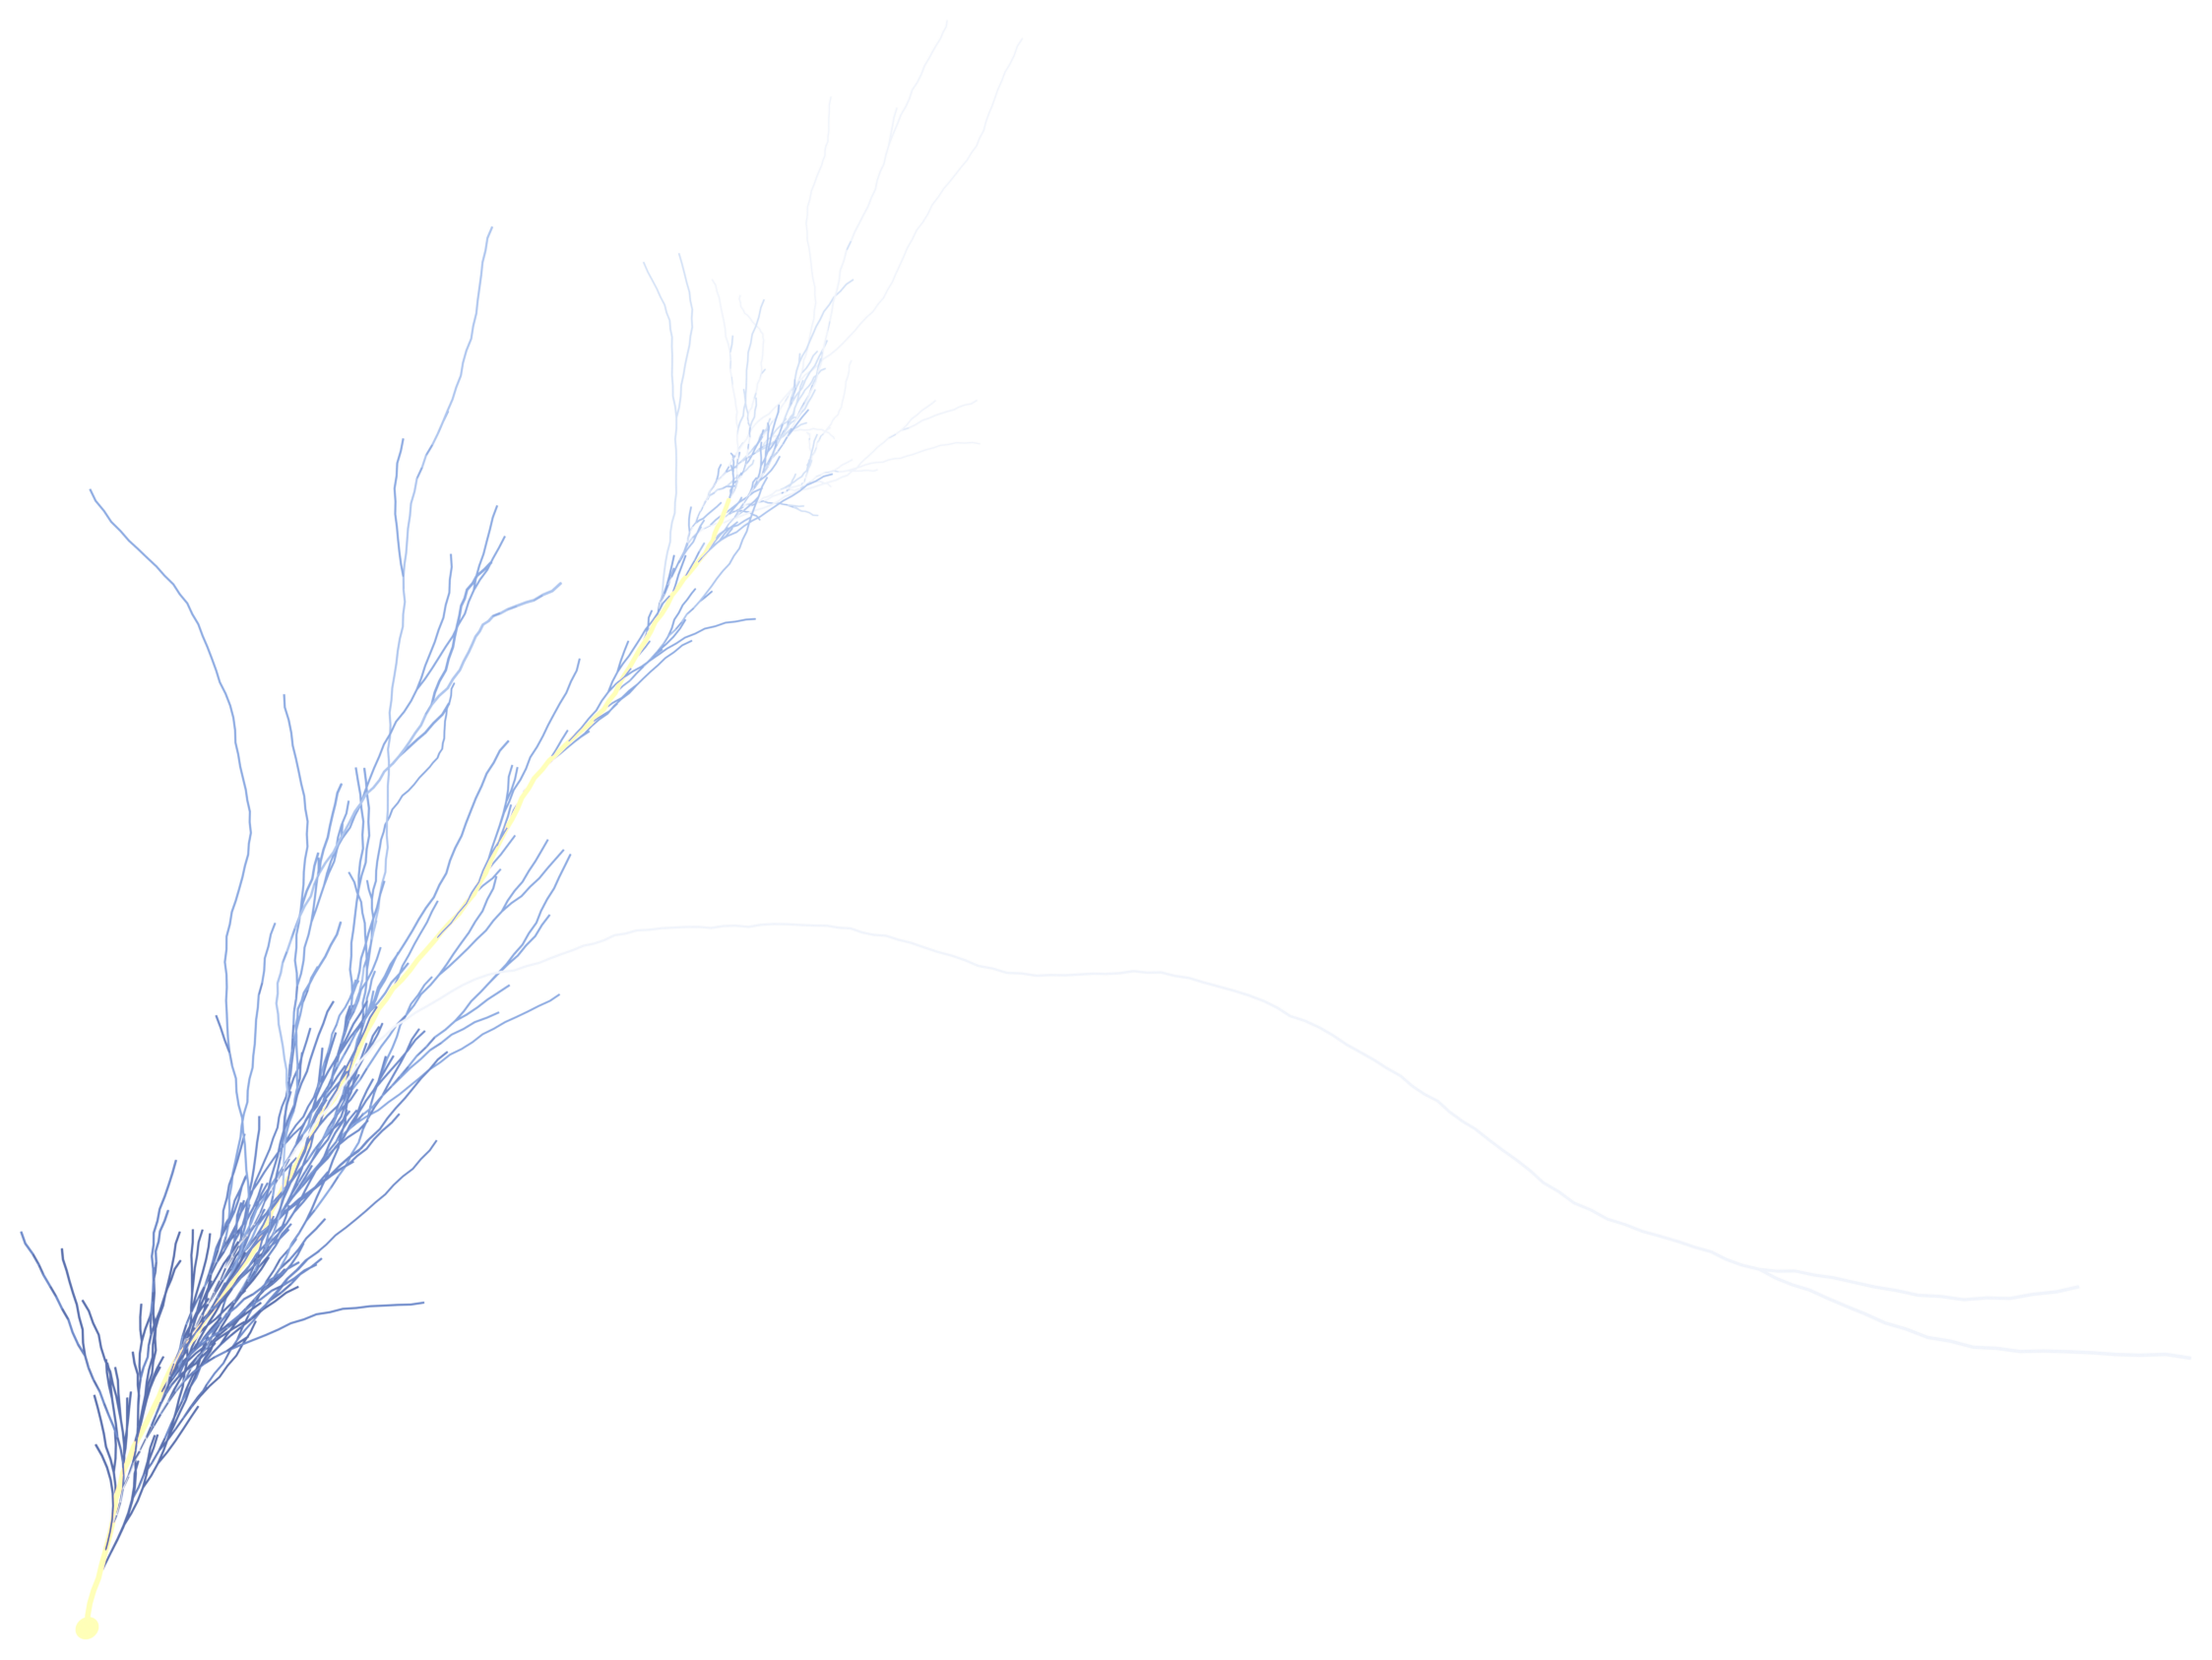
\includegraphics[height=6.6in]{coral_crop.png}};

  % text column
  \node[anchor=north west, inner sep=0, text width=3.4in, align=left] at (1.0,7.3) {%
    {\fontsize{8}{10}\selectfont\color{dim}\textls[180]{\textsc{the collatz conjecture}}\hfill 1937}\par
    \vspace{10pt}{\color{gold}\rule{0.4in}{0.6pt}}\par
    \vspace{13pt}
    {\fontsize{30}{34}\selectfont\color{ink}The\hspace{0.3em}$3n+1$\hspace{0.3em}Problem\par}
    \vspace{13pt}
    {\fontsize{13.5}{17}\selectfont\color{ink}%
      $f(n)=\begin{cases} n/2 & \text{if\ \ }n\text{\ \ is even}\\[2pt] 3n+1 & \text{if\ \ }n\text{\ \ is odd} \end{cases}$\par}
    \vspace{13pt}
    {\fontsize{9.5}{14.5}\selectfont\color{body}%
      Start with any positive integer and apply $f$ again and again.
      Every number ever tried eventually falls into the loop
      \mbox{$4 \to 2 \to 1$}. All numbers below $2^{71} \approx 2.36 \times 10^{21}$
      have been checked by computer, yet no one has proved that every
      number must.\par}
    \vspace{13pt}
    {\fontsize{9.5}{14.5}\selectfont\color{body}%
      \textit{``Mathematics may not be ready for such problems.''}\\[2pt]
      \hspace*{1.2em}--- Paul Erd\H{o}s\par}
  };

  % caption
  \node[anchor=south west, inner sep=0, text width=3.3in, align=left] at (1.0,1.0) {%
    {\fontsize{7.5}{10.5}\selectfont\color{dim}%
      Each strand is one starting number $2 \le n \le 1500$, traced backward
      from~1. Even steps bend one way and odd steps the other, so numbers
      that end alike share a branch.\par}
    \vspace{6pt}
    {\fontsize{7.5}{10.5}\selectfont\color{gold}%
      In gold: $n = 27$, which takes 111 steps and climbs as high as 9232
      before falling to~1.\par}
  };
\end{tikzpicture}
\end{document}
